\documentclass[conference]{IEEEtran}
\IEEEoverridecommandlockouts
\usepackage[T1]{fontenc}
\usepackage[utf8]{inputenc}
\usepackage{amsmath,amssymb,booktabs,graphicx,cite,url,balance,flushend}
\renewcommand{\topfraction}{0.92}
\renewcommand{\dbltopfraction}{0.92}
\renewcommand{\textfraction}{0.06}
\renewcommand{\floatpagefraction}{0.75}
\renewcommand{\dblfloatpagefraction}{0.75}
\setcounter{topnumber}{4}
\setcounter{dbltopnumber}{4}
\setcounter{totalnumber}{6}
\pdfinfo{
  /Title (Component Evaluation of Hybrid A2C-APF Guidance in Wind-Perturbed UAV Simulation)
  /Author (Hieu Ta Chi; Huy Nguyen Anh; Hoa Vu Minh)
  /Subject (UAV navigation with hybrid A2C and artificial potential fields)
  /Keywords (UAV navigation, reinforcement learning, A2C, artificial potential field, trajectory analysis)
}

\title{Component Evaluation of Hybrid A2C--APF Guidance in Wind-Perturbed UAV Simulation}
\author{\IEEEauthorblockN{Hieu Ta Chi\textsuperscript{1}, Huy Nguyen Anh\textsuperscript{2}, Hoa Vu Minh\textsuperscript{3}}
\IEEEauthorblockA{\textsuperscript{1,2}Thuyloi University, Hanoi, Viet Nam\\
\textsuperscript{3}Faculty of International Business, Foreign Trade University, Hanoi, Viet Nam\\
\textsuperscript{1}hieutc@tlu.edu.vn, \textsuperscript{2}huyabcd2004@gmail.com, \textsuperscript{3}k62.2312550029@ftu.edu.vn}}

\begin{document}
\maketitle

\begin{abstract}
Hybrid reinforcement learning and reactive guidance are attractive for cluttered UAV navigation, yet their empirical value is difficult to assess when controller descriptions and evaluation accounting diverge. We present a component evaluation of a guidance controller that blends Advantage Actor--Critic (A2C) with an Artificial Potential Field (APF) in a wind-perturbed point-mass simulation. A2C observes vehicle motion, goal displacement, and wind, whereas the APF channel receives obstacle geometry and contributes reactive guidance through a distance-adaptive blend. The study uses four fixed 300-m environments, five independently trained runs (models) per map for each learned configuration, and 50 deterministic rollouts per run. The hybrid completed all 1,000 rollouts, compared with 830 for a budget- and protocol-matched A2C-only configuration and 55 for APF-only control. Across 20 paired map--training-run units, the A2C-only configuration had a 17-percentage-point lower completion rate ($p=0.027$) and higher finite-difference jerk and acceleration ($p<0.001$ and $p=0.006$, respectively). Differences in successful-path efficiency, clearance, and episode length were not supported. Because the A2C observation carries no obstacle geometry, this comparison evaluates the APF-informed guidance channel together with its privileged obstacle-geometry input rather than isolating potential-field computation. The results demonstrate consistent benefits from that channel under the evaluated simulator and map protocol, while broader generalization and physical-flight relevance remain to be investigated.
\end{abstract}

\begin{IEEEkeywords}
UAV navigation, deep reinforcement learning, A2C--APF guidance, trajectory dynamics, component evaluation.
\end{IEEEkeywords}

\section{Introduction}
Low-altitude navigation in clutter combines three demands: sustained progress toward a goal, collision avoidance, and control behavior that does not vary abruptly under disturbance. A global geometric route can be valuable when a map is known, but closed-loop execution must still respond to local state and perturbations. Conversely, a learned continuous controller can adapt through interaction, yet its safety and reliability depend on training seeds, reward details, observations, and termination logic. These dependencies make implementation alignment especially important in simulation studies: an aggregate result is difficult to interpret unless the reported controller and evaluation procedure match those used in the experiments \cite{henderson2018deep}.

Artificial Potential Fields (APFs) provide inexpensive reactive guidance, but are susceptible to local minima, oscillation, and gain sensitivity \cite{khatib1986real}. Sampling-based methods such as RRT and RRT* address known-map planning under a different information structure \cite{lavalle1998rrt,karaman2011sampling}. Reinforcement learning (RL) instead learns a state-to-action mapping. Combining APF with RL is consequently plausible but not novel by itself: recent work has coupled potential fields with learned UAV search, vortex fields, and PPO-based multi-UAV planning \cite{jin2025hybrid,xiao2025vapf,lee2025apfppo}.

This paper asks a controlled question: \emph{what measurable value does an APF guidance channel add to a fixed A2C navigation implementation?} A2C is used as a compact on-policy reference so that the value added by the analytical channel is easy to attribute, recognizing that this channel also supplies obstacle geometry the learned observation never receives. We make three contributions:
\begin{itemize}
\item a fully specified A2C--APF guidance controller with a 12-dimensional observation, normalized-force semantics, point-mass dynamics, correlated wind, and adaptive action blending;
\item a four-map simulation campaign separating hybrid guidance (H0), a budget- and protocol-matched A2C-only configuration (H1; matched in training budget, maps, and evaluation realizations, but not in obstacle information), APF-only control (H2), and a same-grid interpolation diagnostic (H4); and
\item training-run-level paired analysis and complete outcome accounting that quantify changes in completion reliability and sampled trajectory variation.
\end{itemize}
We do not propose a new reinforcement-learning algorithm or a general path-planning framework. Instead, the study evaluates one APF-informed guidance channel within a fixed A2C implementation. The analysis is restricted to the completed H0, H1, H2, and H4 comparisons; it does not support rankings against PPO, SAC, or RRT.

\section{Related Work}
\subsection{Classical and reactive navigation}
RRT introduced rapid exploration of continuous configuration spaces, while asymptotically optimal sampling-based methods formalized convergence toward optimal paths \cite{lavalle1998rrt,karaman2011sampling}. Recent UAV reviews and hybrid planners continue to show the trade-off between global search, online response, and computational cost \cite{zheng2025uav,li2024gapf}. These planners are useful references for map-based route generation, but are not directly comparable to the present wind-perturbed feedback controller without matched sensing, tracking, and replanning assumptions. APF instead computes local attraction and repulsion online \cite{khatib1986real}. Its low computational overhead motivates its use as a guidance prior rather than a complete planner.

\subsection{Actor--critic control and empirical rigor}
A2C belongs to the advantage actor--critic family, using a critic to reduce policy-gradient variance through value-based advantage estimates \cite{mnih2016a3c}. PPO, SAC, and DDPG are important continuous-control alternatives \cite{schulman2017ppo,haarnoja2018sac,lillicrap2016ddpg}, but algorithm ranking requires algorithm-specific tuning, equal budgets, and multiple training seeds. Deep-RL results can vary substantially with implementation and experimental choices \cite{henderson2018deep}, while real-world learning introduces additional safety and transfer challenges \cite{dulac2021challenges,tobin2017domain}. We therefore use A2C to evaluate the APF-informed guidance channel together with its privileged obstacle-geometry input, not to claim superiority, sample efficiency, or onboard computational advantage. Because the A2C observation carries no obstacle geometry, the H0--H1 contrast does not isolate potential-field computation from the value of the additional obstacle information.

\subsection{Hybrid APF--RL navigation}
Recent APF--RL studies differ in task, potential construction, and integration point \cite{jin2025hybrid,xiao2025vapf,lee2025apfppo}. Potential guidance may shape rewards, constrain actions, or be blended directly with policy output. Related UAV studies also emphasize wind-aware control, disturbance adaptation, and smooth reference generation \cite{wu2024wind,neuralfly2022,datt2021,mellinger2011minimum}. Our design uses direct convex action blending. This makes H0--H1 a transparent component comparison, although it also gives H0 privileged obstacle geometry unavailable to the learned observation. That asymmetry is central to interpretation and should be stated explicitly.

\section{System Model and Controller}\label{sec:method}
\subsection{MDP, observation, and action semantics}
We formulate an episodic Markov decision process $\mathcal{M}=(\mathcal{S},\mathcal{A},P,R,\gamma)$ with $\gamma=0.99$. At time $t$, the implementation exposes
\begin{equation}
s_t=[p_t,v_t,g-p_t,w_t]\in\mathbb{R}^{12},
\end{equation}
where $p_t,v_t,g,w_t\in\mathbb{R}^3$ are position, velocity, goal, and current wind velocity. The RL observation contains \emph{no obstacle geometry or obstacle distance}. Obstacles enter only the APF, reward clearance calculation, collision test, and offline metrics.

The policy action $a_t^{\rm A2C}\in[-1,1]^3$ is a normalized force command rather than an acceleration command. After hybridization, each command component is clipped to $[-1,1]$ and scaled by 12~N; the limit therefore applies per axis, not to the vector norm. Mass, gravity, drag, wind, and integration then determine acceleration. Figure~\ref{fig:architecture} summarizes the closed-loop controller as implemented.

\begin{figure}[t]
\centering
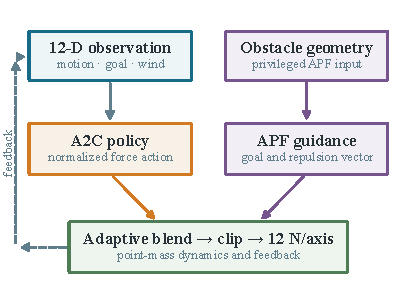
\includegraphics[width=0.88\columnwidth]{figures/controller_architecture.pdf}
\caption{Implemented hybrid controller. The learned observation is 12-dimensional and contains no obstacle geometry; AABB geometry is reserved for APF guidance and collision checks. The adaptive blend uses a distance-dependent $\lambda_t\in[0.15,0.55]$.}
\label{fig:architecture}
\end{figure}

\subsection{Point-mass dynamics}
The simulator uses mass $m=0.5$~kg, linear drag coefficient $k_d=0.12$, gravity $g_0=9.81$~m/s$^2$, and $\Delta t=0.1$~s. For final normalized command $u_t$, the force and acceleration are
\begin{align}
F_t &= 12\,\operatorname{clip}(u_t,-1,1)-m g_0 e_z,\\
a_t &= \frac{F_t-k_d(v_t-w_t)}{m}.
\end{align}
Wind is thus an air velocity inside relative-air-velocity drag, not a force added directly to position. Semi-implicit Euler updates velocity before position:
\begin{align}
v_{t+1}&=v_t+a_t\Delta t,\\
p_{t+1}&=p_t+v_{t+1}\Delta t.
\end{align}
Altitude is clamped to $z\in[5,6]$~m after integration, and vertical velocity is reset to zero when the clamp activates. The model omits attitude, rotor, actuator-rate, and low-level tracking dynamics; commanded force can therefore change much faster than on a physical multirotor.

The initial nominal position is $(0,0,5)$~m and the goal is $(D,0.5D,5)$~m, with a uniformly perturbed reset position of at most $0.5$~m per coordinate before altitude clamping. The distance-dependent horizon is
\begin{equation}
H=\left\lfloor\frac{\|g_{xy}-p_{0,xy}\|}{v_{\rm ref}\,\Delta t}\,1.8\right\rfloor+300,\quad v_{\rm ref}=5~\mathrm{m/s},
\end{equation}
so the nominal 300-m maps have $\|g_{xy}-p_{0,xy}\|=\sqrt{300^2+150^2}=335.4$~m and $H=\lfloor(335.4/0.5)\,1.8\rfloor+300=1507$ transitions. Success requires a final Euclidean goal distance below 3~m and no collision.

\subsection{Obstacle maps and collision semantics}
Obstacles are axis-aligned bounding boxes (AABBs). The evaluation uses four 300-m layouts with density parameter 0.8: a seeded random field, a corridor formed by paired boxes, a two-part barrier with an opening, and a mixed barrier-plus-random environment. Figure~\ref{fig:environment} illustrates the mixed environment in three dimensions and from above. The other layouts broaden the geometric conditions while keeping the main presentation compact. Collision uses a slab intersection test from $p_t$ to $p_{t+1}$, preventing obstacle tunneling between discrete samples. The vehicle inflation radius is zero. Collision is evaluated before success and therefore has outcome priority. Every episode receives exactly one status: collision, success, or timeout.

\begin{figure*}[!t]
\centering
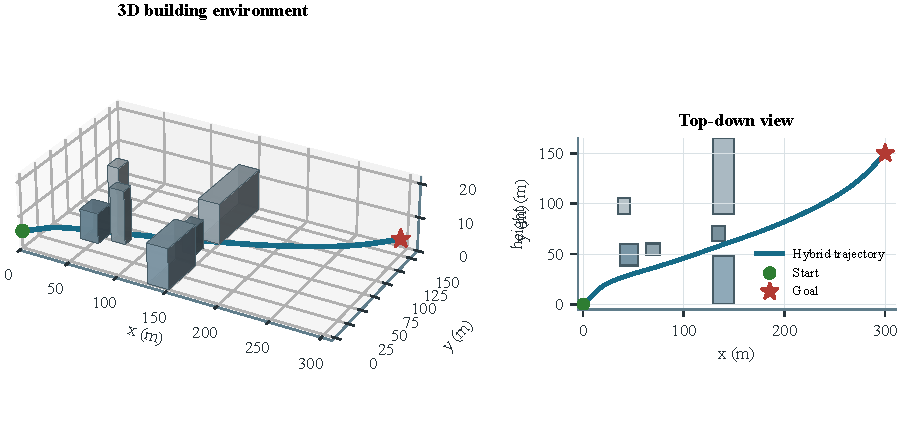
\includegraphics[width=0.84\textwidth]{figures/environment_25d.pdf}
\caption{Representative 3D building environment and top-down projection. The same executed hybrid trajectory is shown in both views, with elevated boxes representing obstacles between the common start and goal.}
\label{fig:environment}
\end{figure*}

\subsection{APF equations and adaptive blending}
The implementation's APF obstacle distance is the Euclidean distance to each AABB \emph{center}, not nearest-surface clearance. For obstacle center $c_i$, goal displacement $q_t=g-p_t$, gains $k_{\rm att}=0.04$, $k_{\rm rep}=18$, and influence radius $d_0=6$~m,
\begin{align}
F_{\rm att}(p_t)&=k_{\rm att}\frac{q_t}{\|q_t\|+\epsilon},\\
F_{{\rm rep},i}(p_t)&=
\begin{cases}
k_{\rm rep}\left(\frac{1}{d_i}-\frac{1}{d_0}\right)\frac{p_t-c_i}{d_i^3},&d_i<d_0,\\
0,&d_i\ge d_0,
\end{cases}\\
d_i&=\|p_t-c_i\|+\epsilon.
\end{align}
The resultant $F_{\rm APF}=F_{\rm att}+\sum_iF_{{\rm rep},i}$ is divided by its norm only when that norm exceeds one, then clipped componentwise to $[-1,1]$. Because center distance can exceed 6~m even when the vehicle is near a large box face, this implementation under-repels wide obstacles; it is not equivalent to nearest-point AABB repulsion and should not be interpreted as such.

The hybrid command is
\begin{align}
u_t&=(1-\lambda_t)a_t^{\rm A2C}+\lambda_t a_t^{\rm APF},\\
\lambda_t&=\operatorname{clip}\left(1-\frac{\|g-p_t\|}{300},0.15,0.55\right).
\end{align}
APF contribution is therefore 0.15 far from the goal and rises to at most 0.55 near it. H1 sets policy mode to A2C and bypasses APF blending; H2 uses APF alone.

\subsection{Reward function}
Let $d_t=\|g-p_t\|$ after the transition, $\delta_t$ be signed AABB surface clearance, and $n_t$ the transition count. The reward is
\begin{equation}
\begin{split}
r_t={}&3(d_{t-1}-d_t)-0.05\\
&-200\,\mathbb{I}_{\rm collision}+B_t\,\mathbb{I}_{\rm success}\\
&+0.3(\delta_t-2)\,\mathbb{I}[2<\delta_t<8]+r_z,
\end{split}
\end{equation}
where collision and success are mutually ordered and
\begin{equation}
B_t=\max\left(80,150\left(1-\frac{n_t}{H}\right)\right).
\end{equation}
The clearance term is positive between 2 and 8~m and increases with clearance inside that band; below 2~m, the reward has no direct proximity penalty apart from collision. The altitude term is $r_z=-15(5-z)$ below 5~m and $r_z=-15(z-6)$ above 6~m. Because altitude is clamped before reward evaluation, this term is inactive during the evaluated transitions.

\subsection{Correlated wind}
At reset, a horizontal base direction is sampled uniformly with magnitude 2~m/s. Gust follows a vector AR(1) process
\begin{align}
\phi&=\exp(-\Delta t/\tau),\quad \tau=0.9~\mathrm{s},\\
\eta_t&=L\xi_t,\quad \xi_t\sim\mathcal{N}(0,I),\\
g_{t+1}^{w}&=\phi g_t^{w}+1.2\sqrt{1-\phi^2}\,\eta_t,\\
w_t&=w_{\rm base}+g_t^{w},
\end{align}
where $LL^\top$ has horizontal cross-correlation 0.35, zero horizontal--vertical correlation, and vertical variance scale 0.09. This AR(1) disturbance is not a validated Dryden spectrum or an urban aerodynamic model. Because the evaluation includes neither a no-wind condition nor additional wind intensities, it does not establish robustness across wind levels.

\subsection{A2C rationale and training configuration}
A2C offers a direct on-policy actor--critic baseline with fewer moving parts than replay-based methods, making component attribution easier. Stable-Baselines3 \texttt{MlpPolicy} is trained on CPU with learning rate $3\times10^{-4}$, rollout length $n_{\rm steps}=256$, $\gamma=0.99$, GAE $\lambda=0.95$, entropy coefficient 0.02, and maximum gradient norm 0.5. Each learned map--seed run uses one environment and five million environment steps. Evaluation uses deterministic policy actions.

Environment and numerical streams are seeded for each run, but A2C does not receive a separate explicit seed. The five training seeds therefore produce distinct trained models and environment streams, although exact rerun determinism across the learning stack is not guaranteed.

\section{Experimental Protocol}\label{sec:protocol}
\subsection{Essential campaign and cardinality}
Table~\ref{tab:design} describes the evaluated campaign. For H0 and H1, four maps and five independently trained runs per map give 20 map--training-run units. Each unit contributes 50 deterministic rollouts (five evaluation-seed labels with ten episodes each), yielding 1,000 descriptive rollouts per learned configuration. Paired inference uses the 20 map--training-run summaries rather than treating all rollouts as independent. H2 follows the same 1,000-row disturbance layout without learning; repeated training-run labels do not represent independent APF controllers. H4 reuses the 1,000 H0 trajectories and performs no control intervention.

\begin{table}[t]
\centering
\caption{Evaluated configurations. H4 is a paired post-processing diagnostic rather than a controller.}
\label{tab:design}
\begin{tabular}{lllll}
\toprule
ID & Type & Maps/units & Train & Rollouts\\
\midrule
H0 & Hybrid & $4/20$ & 5M/unit & 1000\\
H1 & A2C only & $4/20$ & 5M/unit & 1000\\
H2 & APF only & $4/--$ & none & 1000\\
H4 & Diagnostic & same H0 & none & 1000\\
\bottomrule
\end{tabular}
\end{table}

Training seeds are 101, 211, 307, 401, and 503. Evaluation uses base seeds 1009, 1013, 1019, 1021, and 1031, with ten episodes per base seed. Episode seeds are formed by adding the episode index to the base value; because the five ten-wide windows overlap, the 50 combinations reduce to 32 distinct numerical seeds (1009--1040), so 18 of the 50 slots per unit are exact repeats under the deterministic policy. Rates are reported over all 50 slots, as above, but this repetition is a pseudoreplication limitation, and the rollouts are not treated as independent inferential units.

\subsection{Metrics and statistical analysis}
Success and collision rates use complete stored outcome counts. Wilson score intervals describe rollout proportions \cite{wilson1927probable}. Successful-path efficiency is
\begin{equation}
E=\min\left(1,\frac{\|g-p_0\|}{\sum_{t=0}^{T-1}\|p_{t+1}-p_t\|}\right)
\end{equation}
and excludes failures. Minimum clearance is the minimum signed Euclidean AABB surface clearance along the raw executed path; unlike the APF, this metric does use AABB geometry rather than center distance.

From sampled positions, velocity, acceleration, and jerk are finite differences at $\Delta t=0.1$~s. The acceleration index is the mean $\|\Delta^2p/\Delta t^2\|$ and jitter is the mean $\|\Delta^3p/\Delta t^3\|$. These are discrete finite-difference trajectory-variation diagnostics; they do not establish actuator feasibility, motor effort, attitude smoothness, passenger comfort, or physical flight readiness.

Rollouts are nested within 20 map--training-run units. H0--H1 inference therefore uses paired training-run means and two-sided Wilcoxon signed-rank tests, with paired Cohen's $d_z=\overline{\Delta}/s_\Delta$. Efficiency has 18 valid pairs because some H1 training-run units contain no successes. Primary outcomes were not prespecified as a confirmatory family, so the $p$-values across the six component metrics are exploratory and are not multiplicity-corrected; exact $p$-values and effect sizes are therefore emphasized rather than a binary significant/non-significant label.

\subsection{Post-processing diagnostic}
The cubic spline parameterizes each coordinate over normalized sample index and resamples to $\max(20,N)$ points. All H0 trajectories satisfy $N\ge20$, so the output and input have equal sample counts. This operation occurs after rollout and cannot affect actions, collisions, outcomes, or executed path length. H4 compares roughness before and after same-length resampling. Since the spline is evaluated at the original evenly spaced parameter locations, H4 is a numerical post-processing diagnostic rather than a smoothing ablation.

\section{Results}\label{sec:results}
\subsection{Overall outcome accounting}
Aggregate success, collision, and timeout counts are rollout-level descriptive statistics over 1,000 rollouts per configuration; H0--H1 significance instead relies on paired inference over 20 (map, training-run) units. Table~\ref{tab:outcomes} reports all controller outcomes. H0 succeeded in 1,000/1,000 rollouts (Wilson 95\% CI 0.996--1.000) with no collision or timeout. H1 succeeded in 830/1,000 (0.805--0.852), with 58 collisions and 112 timeouts. H2 succeeded in only 55/1,000 (0.042--0.071), colliding 905 times and timing out 40 times.

\begin{table}[t]
\centering
\caption{Rollout outcomes and success-only path efficiency (mean $\pm$ SD).}
\label{tab:outcomes}
\resizebox{\columnwidth}{!}{%
\begin{tabular}{lccccc}
\toprule
Controller & Success & SR (95\% CI) & Collision & Timeout & Efficiency\\
\midrule
H0 Hybrid & 1000 & 1.000 (0.996--1.000) & 0 & 0 & $0.883\pm0.075$\\
H1 A2C & 830 & 0.830 (0.805--0.852) & 58 & 112 & $0.892\pm0.099$\\
H2 APF & 55 & 0.055 (0.042--0.071) & 905 & 40 & $0.882\pm0.041$\\
\bottomrule
\end{tabular}}
\end{table}

At the training-run level, H1 success was 0.17 lower than H0 ($d_z=-0.509$, Wilcoxon $p=0.0273$, $n=20$). This result indicates that APF guidance contributed to reliability under the tested maps and correlated wind process. It should not be interpreted as a safety guarantee beyond these simulation conditions.

\subsection{Map-level reliability and failure structure}
The success gap was strongly map-dependent (Fig.~\ref{fig:outcome-matrix}). H0 achieved 250/250 successes on every map. H1 achieved 250/250 on mixed, 240/250 on corridor, 200/250 on barrier, and 140/250 on random. Its corridor failures were ten collisions; barrier failures were 50 timeouts; and random failures comprised 48 collisions and 62 timeouts. The mixed map's ceiling result shows that APF was not necessary for every fixed layout, while the random and barrier results show where the component mattered most. The same figure separates collision and timeout proportions, making the failure-mode shift explicit: H1's barrier losses are timeouts, whereas H2's losses are predominantly collisions.

H2 succeeded 50/250 times on random and 5/250 on barrier, but never on corridor or mixed. It produced 190, 225, 250, and 240 collisions on random, barrier, corridor, and mixed, respectively. The behavior is consistent with a center-distance APF whose influence radius can fail to activate near broad AABB faces and with the classic limitations of local potential guidance. This mechanistic interpretation is plausible but not proven by a dedicated force-field ablation.

\begin{figure*}[t]
\centering
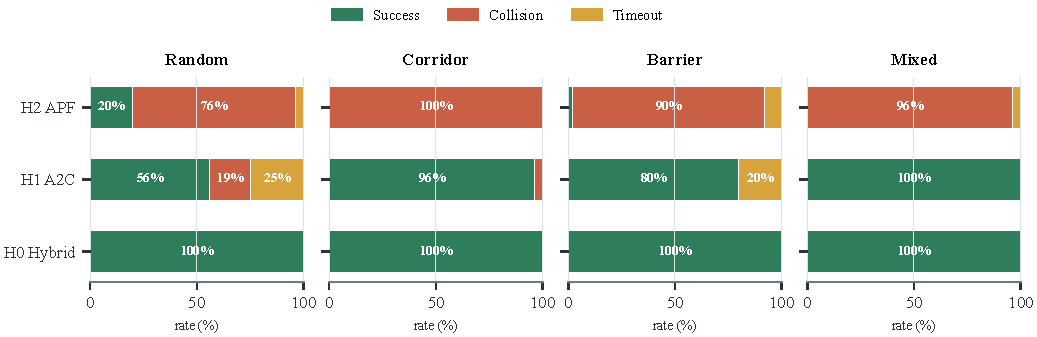
\includegraphics[width=0.93\textwidth]{figures/reliability_by_map.pdf}
\caption{Outcome matrix across the four environments (250 rollouts per cell). H0 succeeds throughout, H1 remains effective but loses reliability on the random and barrier layouts, and H2 predominantly collides before reaching the goal.}
\label{fig:outcome-matrix}
\end{figure*}

\subsection{Path and trajectory dynamics}
\begin{table}[t]
\centering
\caption{Continuous metrics across evaluation rollouts (mean $\pm$ SD). Efficiency is computed only for successful episodes.}
\label{tab:quality}
\resizebox{\columnwidth}{!}{%
\begin{tabular}{lcccc}
\toprule
Controller & Clearance (m) & Steps & Jitter (m/s$^3$) & Accel. (m/s$^2$)\\
\midrule
H0 Hybrid & $7.24\pm5.24$ & $104.4\pm22.7$ & $28.53\pm9.03$ & $16.08\pm1.67$\\
H1 A2C & $7.77\pm6.28$ & $237.8\pm451.3$ & $55.33\pm14.68$ & $22.85\pm7.00$\\
H2 APF & $0.76\pm3.70$ & $408.0\pm339.0$ & $2.21\pm0.82$ & $0.45\pm0.10$\\
\bottomrule
\end{tabular}}
\end{table}

The A2C-only configuration without the APF guidance channel and its privileged obstacle information increased training-run-mean jitter by 26.80~m/s$^3$ ($d_z=1.78$, $p<0.001$, $n=20$) and acceleration by 6.77~m/s$^2$ ($d_z=1.07$, $p=0.006$, $n=20$). Figure~\ref{fig:variation} shows the 20 training-run-paired H1--H0 differences. The pattern is consistent with analytical guidance tempering abrupt learned force commands, although command traces are required to establish the mechanism.

\begin{figure}[t]
\centering
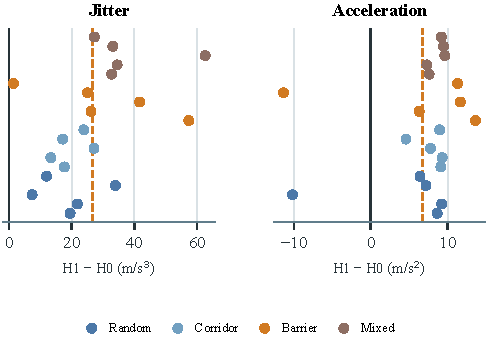
\includegraphics[width=0.90\columnwidth]{figures/paired_dynamics.pdf}
\caption{Paired H1--H0 differences across 20 map--training-run units. Positive values indicate greater sampled trajectory variation without the APF guidance channel. Jitter: $d_z=1.78$, $p<0.001$; acceleration: $d_z=1.07$, $p=0.006$.}
\label{fig:variation}
\end{figure}

The remaining paired differences were not supported: successful-path efficiency had H1--H0 difference $+0.0142$ ($d_z=0.156$, $p=0.417$, $n=18$); clearance $+0.533$~m ($d_z=0.063$, $p=0.956$, $n=20$); and steps $+133.37$ ($d_z=0.300$, $p=0.123$, $n=20$). The raw mean step difference is inflated by long H1 timeouts and high dispersion. We therefore do not claim shorter routes, increased clearance, or faster completion for H0.

H2's low jitter and acceleration do not indicate superior trajectories. They coexist with 90.5\% collision and 4.0\% timeout rates and can result from slow motion or early termination. Comparing roughness without conditioning on task completion would reverse the practical interpretation.

\subsection{Trajectory behavior and map geometry}
The map-level outcome modes provide more information than the overall success rate alone. In the barrier map, H1 produced no collisions but 50 timeouts. The two boxes leave a geometric opening, so this pattern is compatible with failure to maintain sufficient goal progress rather than unsafe penetration. In the corridor, by contrast, all ten H1 failures were collisions. Repeated lateral constraints can expose oscillatory or poorly damped commands even when the target direction is simple. The random layout combined both mechanisms: 48 collisions and 62 timeouts. These distinctions matter because a change that reduces collision without resolving stagnation would not necessarily improve completion, and vice versa.

Figure~\ref{fig:matched-traj} compares the three controllers in separate panels on one barrier layout under the same initial condition and disturbance realization. H0 threads the opening and reaches the goal; H1 takes a long detour and times out; H2 intersects the barrier. The panels make the distinct behaviors behind the aggregate outcome counts explicit.

\begin{figure*}[t]
\centering
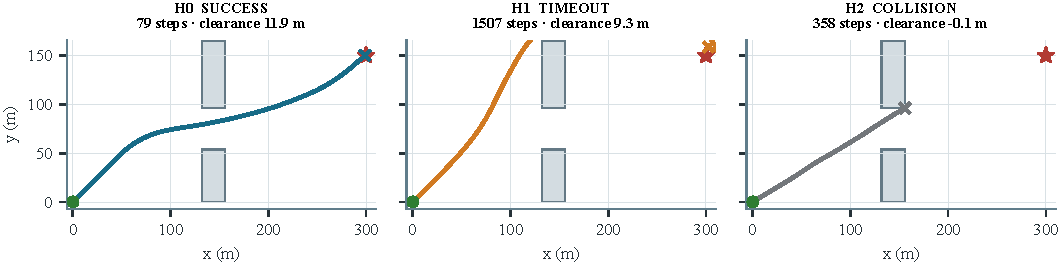
\includegraphics[width=0.98\textwidth]{figures/matched_failure_trajectories.pdf}
\caption{Matched trajectories in the barrier environment. The three panels use the same scale, start, goal, map, and disturbance realization. H0 reaches the goal, H1 times out after a long detour, and H2 collides with the barrier; crosses mark terminal states. The case was selected to illustrate the distinct failure modes found in the aggregate outcomes.}
\label{fig:matched-traj}
\end{figure*}

H0 avoided both H1 failure classes observed in the evaluated rollouts. Its mean of 104.4 transitions corresponds to 10.44~s of simulated time, but this should not be interpreted as a real-flight traversal time: the point mass accepts direct force commands, the altitude band is only 1~m, and no attitude or actuator dynamics constrain the maneuver. H1's mean of 237.8 transitions is similarly difficult to interpret in isolation because its SD of 451.3 reflects the mixture of short successes, collisions, and runs extending toward the 1,507-step horizon. Median H0 and H1 step counts were 99 and 78, respectively. The reversal between means and medians illustrates why ``faster completion'' is not supported by these unconditional episode-length summaries.

Successful trajectories also reveal a trade-off rather than uniform hybrid dominance. H1's rollout-level success-only efficiency mean (0.892) is slightly higher than H0's (0.883), and its mean clearance is also higher (7.77 versus 7.24~m). Neither paired difference is statistically supported. More importantly, conditioning on success removes H1's 170 failures and compares H0 with a selected subset of H1 behavior. The data therefore do not show that APF makes successful paths more direct or more conservative. What they do show is that the hybrid reaches the goal more consistently while exhibiting lower sampled variation.

The APF weighting schedule offers one possible explanation. At the nominal initial goal distance of approximately 335.4~m, $\lambda_t$ is clipped to 0.15. As the vehicle approaches within 255~m of the goal, the unconstrained schedule exceeds this floor; at 135~m it reaches the 0.55 ceiling. Thus the analytical contribution is weakest early and strongest late. Since the force is a convex mixture, this can attenuate large A2C command changes near the terminal region. However, center-based obstacle repulsion is active only within 6~m of a box center, and separate A2C and APF action traces were not recorded. The schedule-based explanation should consequently be treated as a diagnostic hypothesis for future instrumentation.

\section{Discussion}\label{sec:discussion}
The component-level result is consistent across the evaluated maps: adding the APF guidance channel increased completion reliability and reduced sampled trajectory variation. These benefits did not extend to successful-path efficiency or clearance, so the hybrid should not be interpreted as a uniformly superior path planner.

The comparison also contains an important information asymmetry. A2C observes vehicle motion, goal displacement, and wind but not obstacle geometry; H0 receives obstacle centers through APF, whereas H1 does not. H0--H1 therefore measures the value of the complete APF channel, including its privileged geometric input. It does not isolate analytical potential-field computation from additional sensing. A future matched-information study should expose equivalent obstacle features to the learned policy.

H2's failures are compatible with a limitation in the implemented repulsion law. APF activation uses distance to each box center within a 6-m radius, although a box face may be close while its center remains outside that radius. Nearest-surface distance or inflated geometry could better align repulsion with collision risk. This is an implementation-based explanation, not a demonstrated causal result. Likewise, lower finite-difference acceleration and jerk characterize sampled simulator trajectories; without attitude, actuator, and command-rate dynamics they do not establish physical flyability.

\section{Threats to Validity}
Success uses a 3-m endpoint tolerance with collision priority. Reward and clearance use signed AABB surface distance, whereas APF uses center distance; the two obstacle-distance constructs are not interchangeable. Acceleration and jerk are finite differences of sampled positions rather than aerodynamic load, motor effort, or comfort measures.

H0 and H1 share training budgets and map--training-run structure but not obstacle information. Environment streams are seeded, but A2C does not receive a separate seed, so exact rerun determinism is not guaranteed. Fifty declared evaluation combinations map to 32 unique numerical seeds per training run. No logged decomposition of A2C and APF commands establishes the cause of lower variation.

Rollouts are correlated within maps and training runs, so inference uses 20 paired map--training-run units; Wilson intervals remain descriptive. Efficiency is success-only and available for 18 pairs, which introduces survivor-composition differences. H2 labels do not represent independent learned agents, and multiple reported outcomes are not multiplicity-adjusted.

External validity is limited to four fixed 300-m AABB maps and one correlated wind process. The point-mass model omits attitude, rotor dynamics, perception, localization error, latency, energy, and hardware constraints. No held-out-map, wind-level intervention, hardware-in-the-loop, or physical-flight evidence is included, and no ranking claim is made for PPO, SAC, or RRT.

\section{Conclusion}
This study evaluated an APF-informed guidance channel within a fixed A2C controller across four wind-perturbed UAV simulations. H0 completed all 1,000 rollouts, versus 830 for the budget- and protocol-matched A2C-only configuration and 55 for APF-only control. Paired map--training-run analysis supports higher completion reliability and lower finite-difference acceleration and jerk, but not differences in successful-path efficiency, clearance, or episode length. The result reflects the evaluated APF-plus-geometry channel rather than a new learning algorithm or a generally superior planner: H0 receives obstacle information unavailable to H1, and APF repulsion uses obstacle centers. Future work should evaluate held-out maps, matched obstacle observations, surface-distance guidance, varied wind levels, component-action logs, and higher-fidelity or hardware validation.

\appendix
\section{H4 Post-Processing Check}
H4 is not a controller or smoothing ablation. Same-grid cubic-spline resampling of the 1,000 executed H0 trajectories leaves jitter and acceleration unchanged to numerical precision and cannot affect actions, outcomes, or paths; meaningful smoothing evidence would require altered references or grids followed by closed-loop feasibility evaluation.

\bibliographystyle{IEEEtran}
\bibliography{references}
\end{document}
